\documentclass[10pt,conference,compsocconf]{IEEEtran}

%\usepackage{times}
%\usepackage{balance}
\usepackage{url}
\usepackage{graphicx}
\usepackage{subfigure}	% For figure environment

\newcommand{\figref}[1]{Figure \ref{#1}}
\newcommand{\image}

\begin{document}
\title{Road Segmentation from Satellite Images using\\Support Vector Machine Classification}

\author{
  Daniel Val\'erio Sampaio, Yves Bieri\\
  Department of Computer Science, ETH Zurich, Switzerland
}

\maketitle

\begin{abstract}
	
\end{abstract}

\section{Introduction}

The goal of this paper is to introduce a new road segmentation algorithm for urban areas from satellite images. Road detection is important for several applications from autonomous driving to tracking
of road change and urban planning.

The idea of road segmentation is not a new one and has been implemented numerous times, although with
different success. The great difficulty in urban areas is the occurrence of trees and cars partially blocking the view on roads and thus making detection much harder. Additionally parking lots and railways have a lot of identical features to roads which leads to them being misclassified.

Our approach consists of extracting 16 features from out satellite images and using those to build a Support Vector Machine (SVM) classification model. Our features contain the original image, a smoothed version of said image and a region map, based on a skeletonization approach using an euclidean-like distance map, to reveal the underlying road structure.

The image preprocessing and feature extraction is implemented in \emph{python} with the help of mostly \emph{numpy} and \emph{cv2}. Afterwards the features are fed to MATLAB which is used to produce our SVM classifier. We decided on this approach because \emph{MATLAB} is faster and easier to run on the ETH cluster. The predicted results are then fed again to our \emph{python} program for post-processing and to produce our final results.

In section XXX we describe the idea used in our approach in more detail,
followed by the implementation in section XXX and results in section XXX.
Lastly we conclude the paper with a discussion of our work in section XXX and 
give ideas for future work and improvement.

\section{Models and Methods - Feature Extraction}
To detect roads from satellite images we decided to use Support Vector Machines (SVM) for classification. We were given 100 training images with corresponding ground truth, which we used to classify 50 test images in a second step.

For the data-driven classifier to be effective, we decided on a set of key features which we extracted from both the training images and the test images. Contrary to our initial implementation, we decided to not consider every single pixel in the image but to form patches instead. We mostly worked with 4x4, 5x5 and 10x10 patches and eventually decided on keeping the 5x5 patching, which offered a good computational speedup without loosing a lot of information of the image features.

The training and test images were taken from urban areas, which apart from roads contain mostly buildings, trees and cars. A road is a long and compared to its length thin object, often in horizontal or vertical direction and colored in a shade of gray. By concentrating on those key characteristics of a road we build a set of features which we will extract to train our model.

\subsection{Original Image}
The first feature we use is the color in the image patch. It is only natural to include this feature, as a road is usually gray. We can decide whether an image patch is gray by looking at its \emph{RGB} values. They not only help us to find roads that look gray, but also let us recognize different objects in other colors. On one of the images for example there is a pool next to a house, which naturally is blue. Of course, blue objects cannot be roads, and are therefore excluded right from the beginning. In contrast, if the values of red, blue and green all are approximately the same, the resulting color is some kind of gray. So adding the color is a first useful feature to build our model. 

\subsection{Smoothed Image}

As a second feature we decided to add the standard deviation of the color. We stated earlier, that a pixel is gray, if its three \emph{RGB} values are close. This means that if the standard deviation is small, the red, blue and green values are all close together which is a strong indicator that the pixel is gray.

\begin{figure*}[t]
	\centering
	\subfigure[original\label{fig:original}]
	{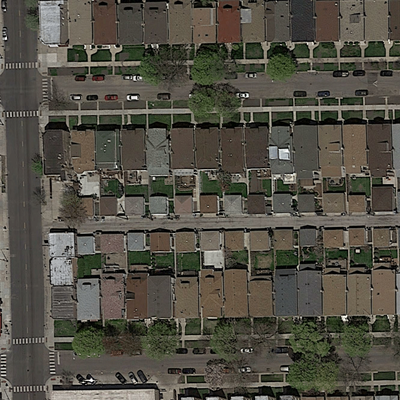
\includegraphics[width=0.38\linewidth]{pics/original.png}}
	\hspace{0.05\linewidth}
	\subfigure[mean-shift filtered \label{fig:mean-shift-filtered}]
	{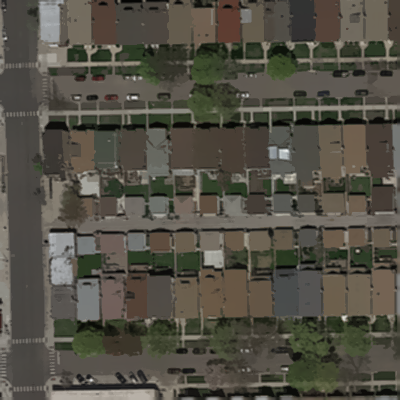
\includegraphics[width=0.38\linewidth]{pics/mean_shifted.png}}
	\caption{Smoothing the original image}
\end{figure*}

After a few trial runs on the training images we noticed that there are a lot of small imperfections which perturb our results. Cars, trees and shadow lead to a pretty big error rate. We concluded that we have to smoothen the images to get rid of this source of noise.

To do that, we used a mean-shift filter, also used in a previous work by Banerjee at al.\cite{BaBuMo12}. This filter allows for edge preserving smoothing of our image, which is essential, considering that roads have distinct borders. For a neighborhood around the pixel the new spatial center and mean color value are calculated and at the end assigned to the pixel. As parameters we used a spatial radius and a color distance of $10$, which seemed to produce reasonably good results in our experiment.

In addition to the previous mean and standard deviation \emph{RGB} values of the original image, we added the ones obtained by the mean-shift filtered image as our third and fourth parameters of our feature vector. 

Besides the original image we also wanted a smoothed version with less noise, as we are convinced that the combination of those two pictures are a good basis for road detection.

\subsection{Region Map}
Our last, and most complex feature is based on the paper by Gaetano et al. \cite{GaZeScPo11}. The morphological analysis the paper is based on assumes that roads are objects that spread over a rather large part of the image and that have a comparatively small width compared to their total length. Building a morphological skeleton is then the base of the algorithm and consequently for this feature. Ideally a road can afterwards be approximately represented by a branch of the skeleton.

Lets take a look at a brief overview of the algorithm:
\begin{enumerate}
	\item Edge Detection
	\item Distance Map
	\item Skeleton
	\item Skeleton Pruning
	\item Road Reconstruction
	\item Watershed Transformation
\end{enumerate}
First edge detection is conducted on the image. The result is then used to compute an euclidean-like distance map (EDM) which then is used to extract the morphological skeleton. Skeletonization although is not very robust, making it therefore desirable to improve it in a post-processing step. To do that, firstly the lines are thinned to a one-pixel width. As we still have too much noise, we also need to remove small branches that are very unlikely to be part of a road. This step is called skeleton pruning. Finally double thresholding is applied to classify valid branches in the skeleton. We consider the average distance in the distance map of every pixel in a skeleton branch and also the overall average distance of every pixel. In the end a watershed transform is applied to reconstruct an image containing various regions, indicating if there is a possible road or not.

\subsubsection{Implementation Details} \hspace*{\fill}

The first step is edge detection. Here, we used a \emph{python} implementation of the canny edge detector, where we first transformed the original into a gray-scale image. Although canny edge detection has a higher computational burden than e.g. a sobel edge detector, we decided to use canny, as the results were more accurate.

\begin{figure*}[tp]
	\centering
	\subfigure[canny edge detection\label{fig:edge_detection}]
	{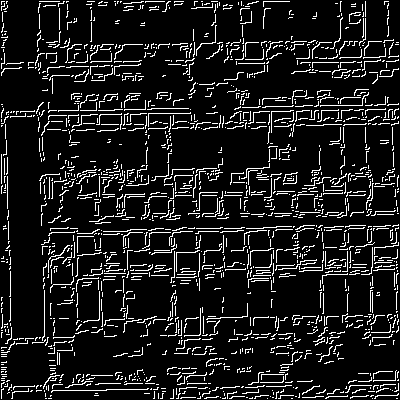
\includegraphics[width=0.30\linewidth]{pics/edge_detection.png}}
	\hspace{0.025\linewidth}
	\subfigure[distance map\label{fig:distance_map}]
	{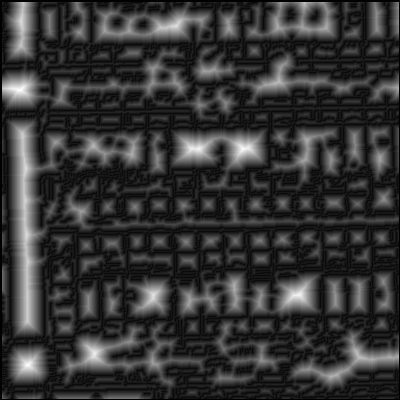
\includegraphics[width=0.30\linewidth]{pics/distance_map.png}}
	\caption{Building the Distance Map}
\end{figure*}

\begin{figure*}[tp]
	\centering
	\subfigure[thinned skeleton\label{fig:skeleton}]
	{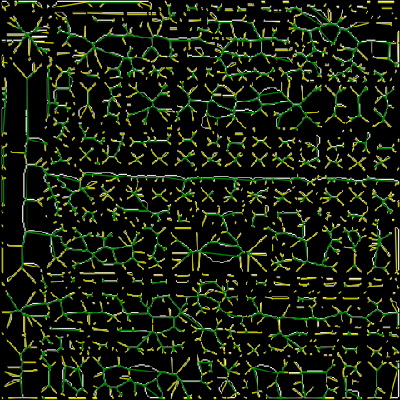
\includegraphics[width=0.28\linewidth]{pics/skeleton.png}}
	\hspace{0.025\linewidth}
	\subfigure[pruned skeleton\label{fig:skeleton_pruned}]
	{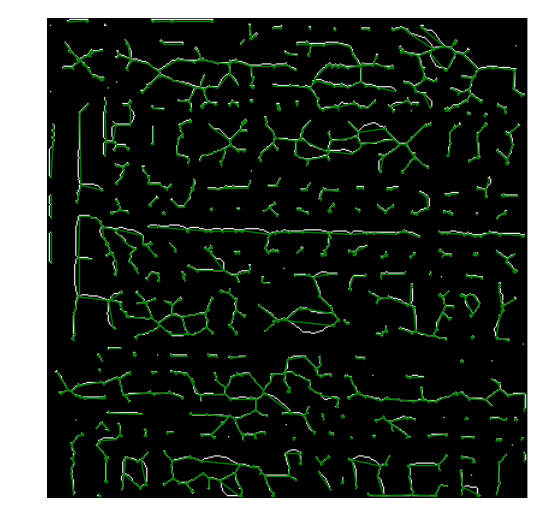
\includegraphics[width=0.28\linewidth]{pics/skeleton_pruned.png}}
	\hspace{0.025\linewidth}
	\subfigure[final skeleton\label{fig:skeleton_final}]
	{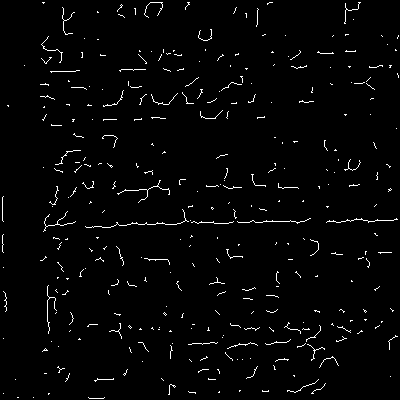
\includegraphics[width=0.28\linewidth]{pics/skeleton_final}}
	\caption{Pruning the Skeleton Map}
\end{figure*}

In the second step we prepare for the morphological skeletonization. With help of the previously generated edge map we create an euclidean-like distance map. We start out by giving all edge pixels from the canny edge map a distance of 1. For the future development of the distance map we consider the 8-neighborhood of each edge pixel (8-neighborhood meaning the 8 pixel that form a one-pixel wide border around the center pixel). The four horizontal and vertical neighbors are given a distance of +1, meaning that if the center pixel had distance 1, they get assigned distance 2. For the four diagonal pixels we add $\sqrt{2}$ to the center pixel's value. By assigning a higher value to the diagonal pixels we generate smoother curves and preciser distance values for further computations. We continue those steps iteratively until all pixels are assigned a value. From now on we refer to the result of this step as the euclidean-like distance map (EDM).

Now, in the third step, we create the morphological skeleton out of our EDM. For this we use a crest line following approach, as described in paper \cite{GaZeScPo11}. With the crest line approach we want to find a relatively simple skeleton. One single straight line is enough to represent a road pretty accurately. As in urban areas most roads are either horizontal or vertical without curves this approach gives us a pretty good result. 

Now we look at all points in the EDM which have a maximum of two neighbors with higher value. These points are considered crest line points. With this approach we recursively add the neighboring points with the steepest ascent to our crest line. Finally we apply morphological thinning to reduce our skeleton to a one-pixel width.

The fourth step consists of pruning the skeleton, as the road skeleton obtained in step 3 has a lot of small branches that most likely are not part of a road. They therefore generate more noise than benefit to the scene, creating a more splintered final image. By pruning the skeleton we can enhance the representation of our roads by getting rid of some of this splintering. As you can see in our skeleton map in \figref{fig:skeleton} we mark all leave nodes and their connections yellow and all intersection nodes as well as their connections to other intersection nodes in green. Finally we consider all nodes with connection degree of one or lower, i.e. all nodes and connections in yellow, and remove those nodes together with the edge/branch.

In the final and concluding step we do road detection and map reconstruction. For this we use a double thresholding method. Recall that we can describe a road as a branch of the skeleton with a large length compared to its width. 

Therefore we can introduce two main cost/score functions, that we will later use for thresholding. The first score is an average over the distance map on the skeleton branch's points $S_{i}$
$$
\{D_i\}_{avg} = \sum_{p \in S_{i}}{\frac{\textrm{EDM}(p)}{\textrm{card}(S_{i})}},
$$
where $i$ indicates the $i$-th skeleton branch. The second one is the so-called road skeleton score (RSS):
$$
RSS_{i} = \frac{{\{D_i\}}_{avg}}{\textrm{card}(S_{i})}
$$
The paper on which the method is based on \cite{GaZeScPo11} proposes to set the threshold to $threshold_{RSS} = 0.04$ and $threshold_{D} = 12$. The points in the skeleton satisfying both conditions, i.e. having a score below these thresholds, are then kept for the final skeleton.

Lastly we apply a marker based watershed transform on the distance map with the proposed skeleton to reconstruct a region map. The watershed transformation summarizes large common patches that we color with the help of our constructed mean-shift filtered image in every single region. Finally we obtain a segmented region map where each connected component contains exactly one connected skeleton segment. 

\subsection{Results}

Such work, much wow! :-)

\section*{Acknowledgements}
The authors thank the producers of Game of Thrones for being such an inspiration in the early mornings about how to kill people in hard times, when things do not go as expected.

\bibliographystyle{IEEEtran}
\bibliography{howto-paper}
\end{document}
